\documentclass{article}
\usepackage[left=2cm,right=2cm,top=2cm,bottom=2cm]{geometry}
\usepackage[utf8]{inputenc}
\usepackage[german]{babel}
\usepackage{amsmath}
\usepackage{dsfont}
\usepackage[export]{adjustbox}
\usepackage{amsthm}
\usepackage{color}
\usepackage{amsfonts}
\usepackage{amssymb}
\usepackage{wasysym}
\usepackage{makeidx}
\usepackage{graphicx}
\usepackage[colorlinks=true,urlcolor=blue,linkcolor=blue]{hyperref}
\usepackage{ziffer}
\usepackage{minted}
\usepackage{xcolor}
\usepackage{framed}
\usepackage{mdframed}
\usepackage{subfiles}
\usemintedstyle{emacs}

\definecolor{purp}{HTML}{9A72AC}
\definecolor{re}{HTML}{FC6255}
\definecolor{gre}{HTML}{83C167}
\definecolor{blu}{HTML}{58C4DD}
\definecolor{shadecolor}{rgb}{0.85,0.85,0.85}
\definecolor{bg}{rgb}{0.95,0.95,0.95}
\setlength{\parindent}{0em} 

\BeforeBeginEnvironment{minted}{\begin{mdframed}[linewidth =2 ,backgroundcolor=bg , linecolor=black, linewidth=0.5]}
\AfterEndEnvironment{minted}{\end{mdframed}}

\newtheorem{defi}{Definition}
\BeforeBeginEnvironment{defi}{\begin{mdframed}[linewidth =2 ,backgroundcolor=bg , linecolor=black, linewidth=0.5]}
\AfterEndEnvironment{defi}{\end{mdframed}}

\newcommand{\bsp}{\textbf{Beispiel}:}
%\newcommand{\task}{\textbf{Aufgabe}:}

\newcommand{\bol}[1]{\textbf{#1}}
\newcommand{\q}[1]{\glqq #1\grqq}
\newcommand{\DODO}[1]{\textbf{\textcolor{red}{DODO:}} #1 \\ \begin{center}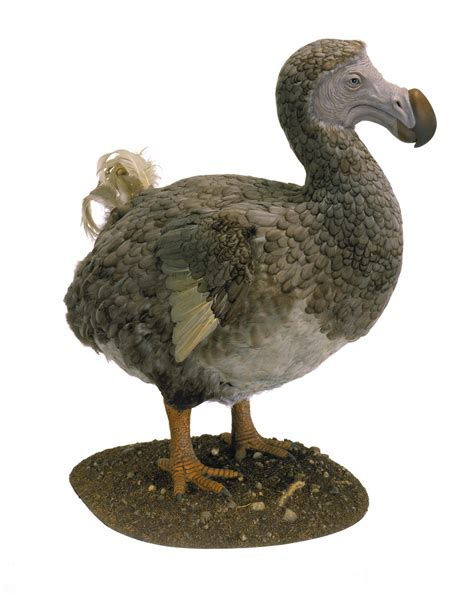
\includegraphics[scale=0.2]{../../media/dodo.jpg} \end{center}}

\newenvironment{task}[1]{
    \begin{shaded*}
    \textbf{Aufgabe #1}:
}{
    \end{shaded*}
}

\begin{document}

\subsection{Einleitung}
Auch der Begriff des Graphen ist - wie auch der Baum - bereits Thema in der 7. Jahrgangsstufe! Ein typisches Beispiel für einen Graphen ist hier die Struktur einer Website bzw. später allgemein des Internets. Die betrachteten Graphen werden hier z.B. so dargestellt: 
\begin{center}
    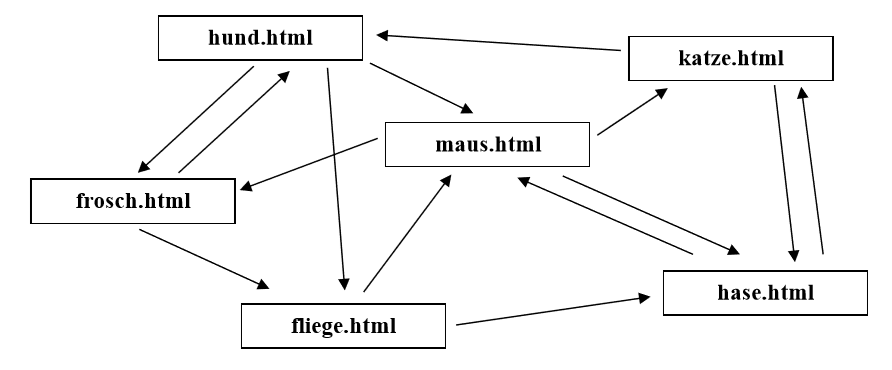
\includegraphics[scale=0.5]{../../media/website.png}
\end{center}
Jeder \textbf{Knoten} stellt hier eine HTML-Datei dar, die Pfeile (\textbf{Kanten}) zeigen eine Verlinkung an - häufig wird statt zwei Pfeilen auch ein Pfeil mit zwei Spitzen verwendet, wenn die Beziehung in beide Richtungen gültig ist. \\
Ein weiteres typisches Einsatzgebiet von Graphen sind Verbindungen zwischen Orten, z.B. beliebig auf einer Karte:
\begin{center}
    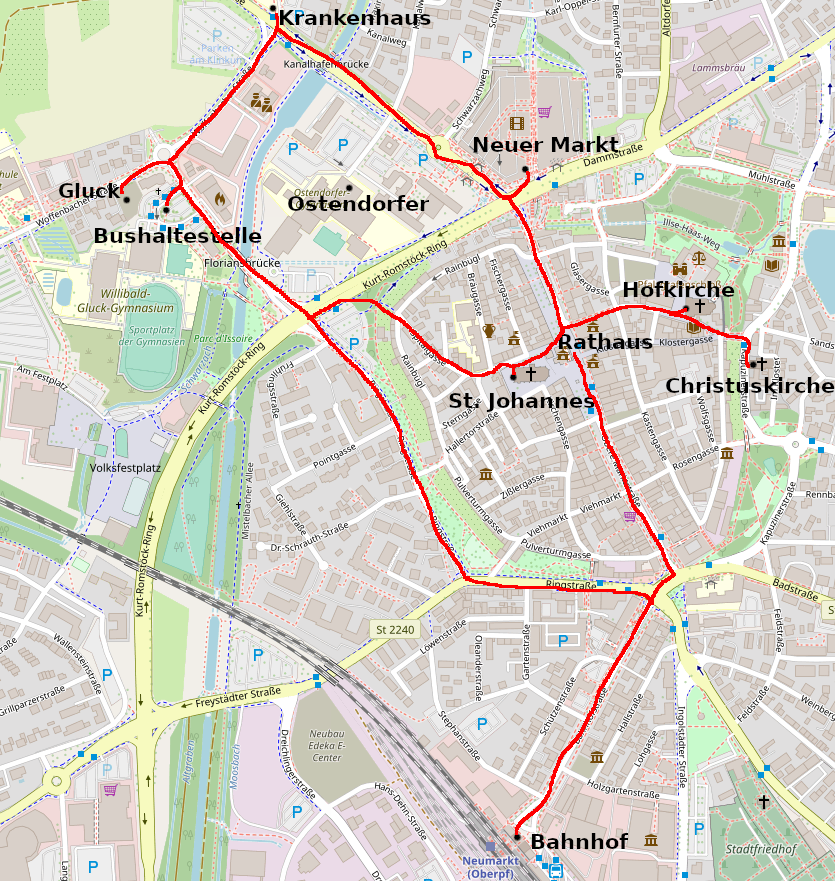
\includegraphics[scale=0.45]{../../media/neumarkt.png}
\end{center}
Hier entspricht jeder Ort von Interesse einem Knoten und die Verbindungswege entsprechen den Kanten - hier ergeben sich bereits die ersten Modellierungsfragen, z.B.:
\begin{itemize}
    \item Welche Orte sollen Knoten werden?
    \item Sollen Orte verbunden werden, wenn es einen Weg gibt?
    \item Falls es mehrere Wege gibt, welcher wird repräsentiert? Der kürzeste oder der \q{schnellste}? (siehe Navigationsprogramme!)
    \item etc.
\end{itemize}
Je nach Modellierung können dann verschiedene Probleme gelöst werden, z.B. die oben bereits erwähnte Routensuche nach dem kürzesten (oder schnellsten) Weg. \\
Ist die Situation spezieller, so werden manche Fragen automatisch von den Gegebenheiten beantwortet, im Folgenden findet sich beispielsweise ein Plan des U-Bahn-Netzes von münchen: 
\begin{center}
    \includegraphics[scale=0.5]{../../media/ubahn_münchen.png}
\end{center}
Modelliert man diese Situation als Graph, so ist offensichtlich jeder Knoten eine Station, jede Kante eine Verbindungsstrecke zwischen zwei Stationen - hier gibt es in der Regel nicht mehrere Wege dazwischen! \\
Die Graphentheorie ist aber nicht auf \q{Wegeprobleme} beschränkt, weitere Beispiele:
\begin{itemize}
    \item \textbf{Soziale Netzwerke}: Graphen können auch Beziehungen zwischen Menschen modellieren.
    \item \textbf{Computernetzwerke}: Ein Graph kann auch z.B. ein lokales Netwerk repräsentieren.
    \item \textbf{Datenbanken}: Modellierung von Zusammenhängen von Daten.
    \item \textbf{\q{Reale Situationen}}: z.B. Modellierung eines Rohrsystems in einem Gebäude zur Analyse von notwendigen Pumpen.
    \item etc. 
\end{itemize}

\subsection{Grundbegriffe}

Zurück zu den Anfängen:
\begin{defi}
Ein Graph ist eine Datenstruktur, die eine Menge von Objekten (Knoten - Nodes) repräsentiert, sowie deren Verbindungen (Kanten - Edges).
\end{defi}
Diese Definition macht klar, dass ein Graph im Wesentlichen eine Verallgemeinerung eines Baumes ist, es gibt jetzt keine Einschränkungen mehr bezüglich der Anzahl der Kinder und auch keinen ausgezeichneten Wurzelknoten. Dadurch verlieren wir zwar auch Vorteile, sind in der Modellierung aber wesentlich offener. \\

Die wichtigsten (offensichtlichen) Eigenschaften bzw. Forderungen an Knoten und Kanten sind:
\begin{itemize}
    \item es gibt nur eine endliche Anzahl an Knoten und Kanten 
    \item jede Kante verbindet genau zwei Knoten 
    \item Knoten und Kanten können jeweils noch Zusatzinformationen verwalten
    \item Zwischen zwei Knoten kann es Kanten \q{in beide Richtungen} geben, dies ist aber nicht zwingend notwendig. 
    \item Knoten und Kanten werden idealisiert dargestellt (z.B. Wegeanalyse: auch wenn ein Weg zwischen zwei Orten \q{kurvenreich} ist, werden die beiden Knoten mit einer geraden Linie verbunden, die Länge des Weges kann dann z.B. im \textbf{Kantengewicht} gespeichert werden, siehe unten.)
\end{itemize}
Wir betrachten das untenstehende Beispiel:
\begin{center}
    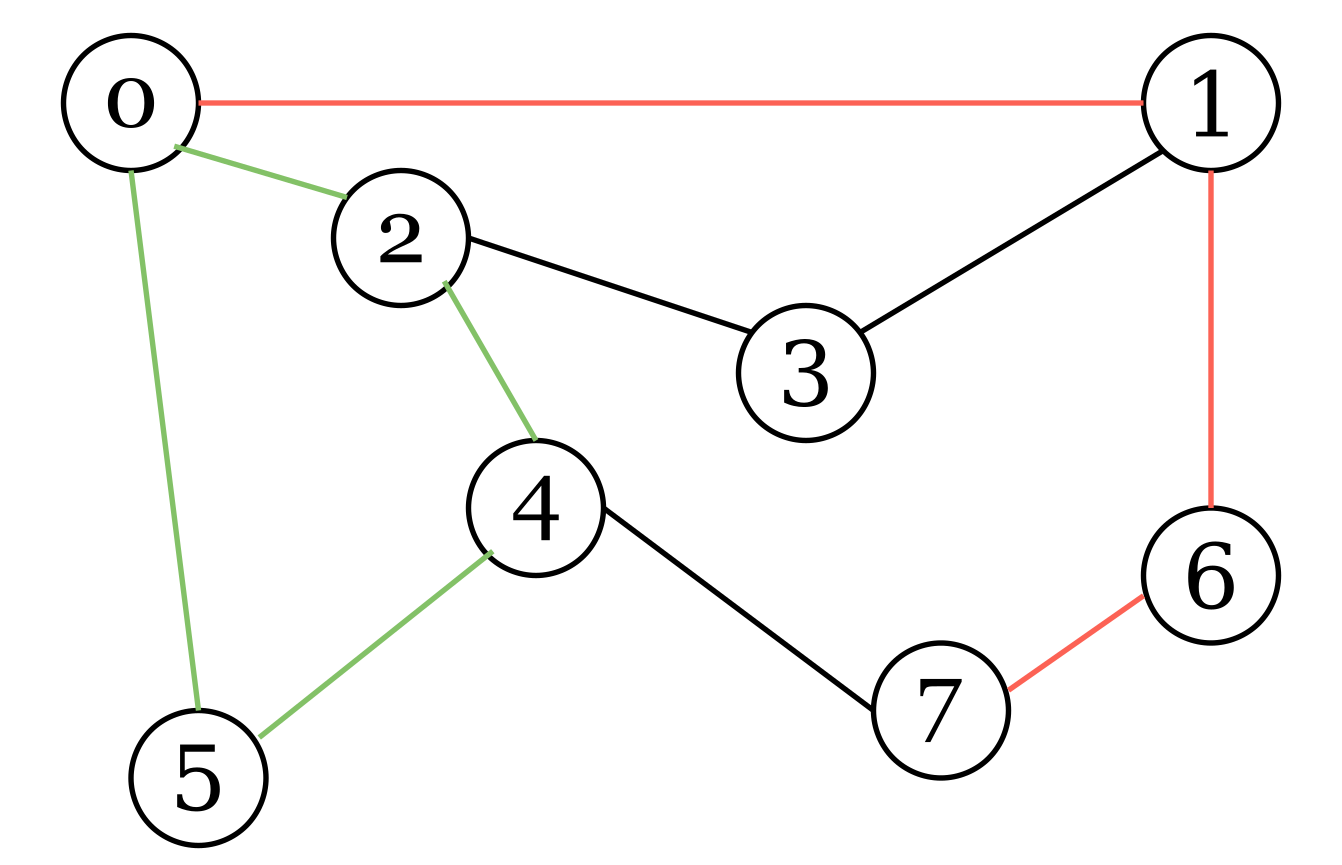
\includegraphics[scale=0.25]{../../media/example_graph.png}
\end{center}
Ein Weg von einem Knoten zu einem anderen Knoten wird \textbf{Pfad} genannt, wenn es eine endliche Folge aufeinander folgender, durch entsprechende Kanten miteinander verbundene Knoten gibt. Wenn dabei kein Knoten mehrfach besucht wird, so spricht man von einem \textbf{einfachen Pfad}. Im obigen Beispiel wäre \color{re} 0 1 6 7 \color{black} ein einfacher Pfad. 
Ist in einem Graph ein \q{Rundlauf} möglich, so spricht man von einem \textbf{Zyklus}. Im obigen Graphen gibt es beispielsweise den Zyklus \color{gre} 0 2 4 5 \color{black}. Im Wesentlichen ist ein Zyklus also ein Pfad, dessen Start- und Endknoten identisch sind.
\vspace{2mm}
\textbf{Weitere wichtige Fachbegriffe}
\begin{enumerate}
    \item \textbf{gerichtet vs. ungerichtet}: Selbsterklärend :) Beispiel:\begin{center}
        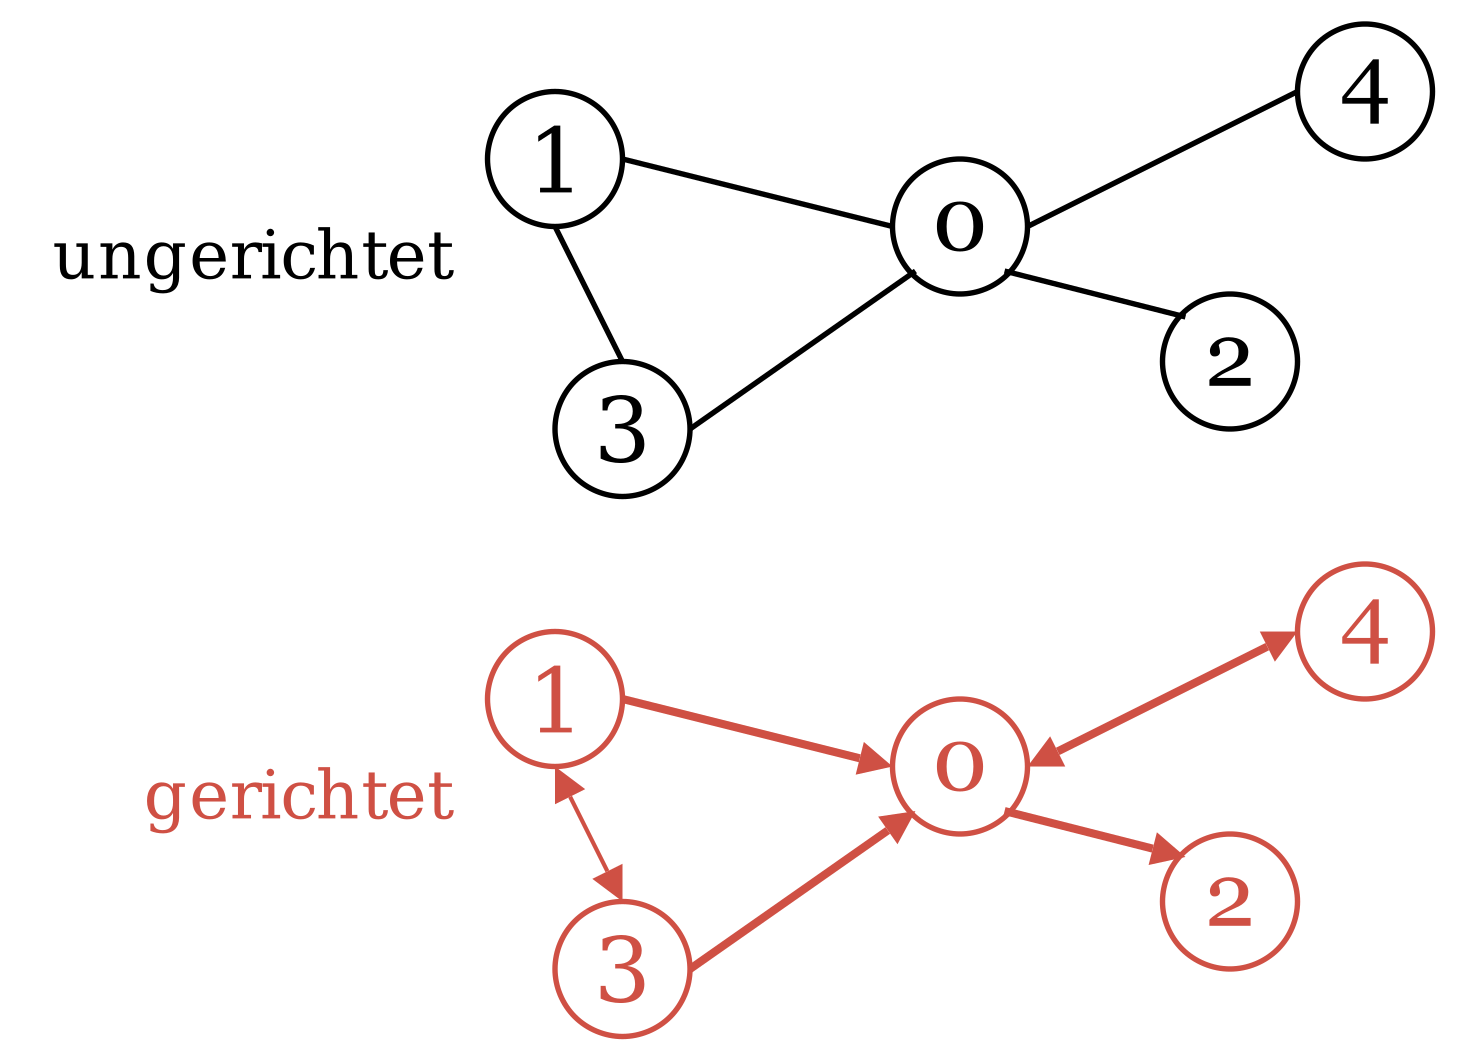
\includegraphics[scale=0.15]{../../media/ungerichtet_gerichtet.png}
    \end{center}
    \item \textbf{gewichtet vs. ungewichtet}: Die Kante eines Graphen kann einerseits bedeuten, dass die beiden Knoten \q{nur} verbunden sind, andererseits kann sie aber auch eine konkrete (physikalische) Größe repräsentieren. In unserem U-Bahn-Beispiel könnten die Kanten Fahrtzeiten in Minuten oder Entfernungen in km darstellen. In einem sozialen Netwerk könnte ein Kantengewicht die Interaktionsfrequenz zweier Menschen beschreiben, usw.: \begin{center}
        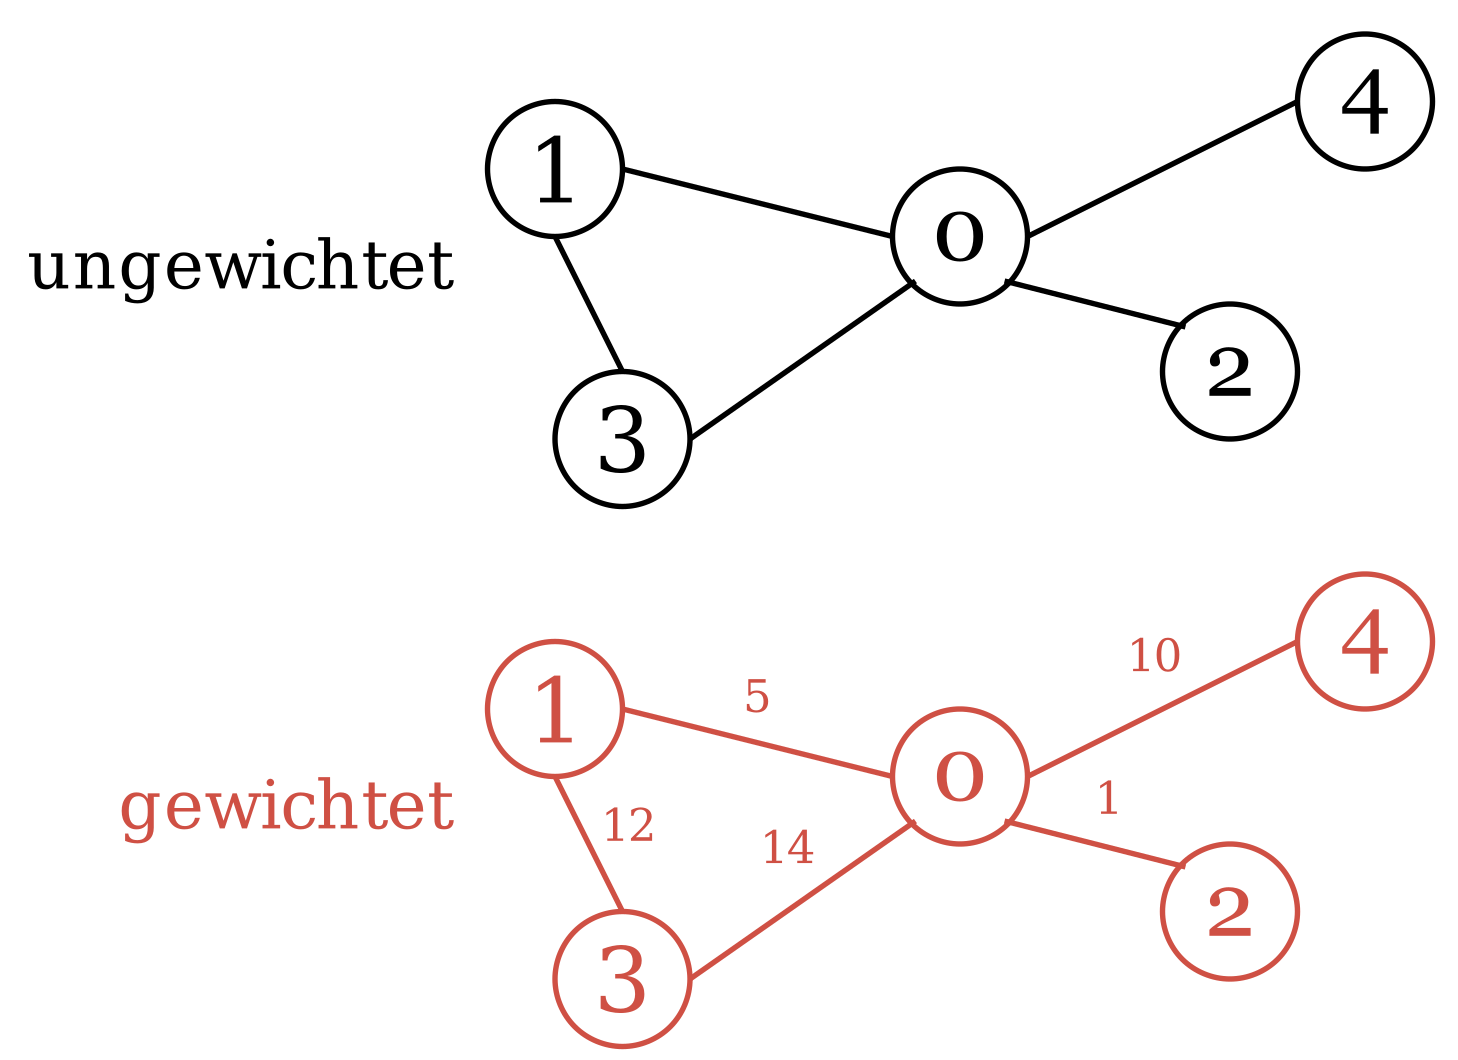
\includegraphics[scale=0.15]{../../media/gewichtet.png}
    \end{center}
    \item \textbf{zyklisch vs. nicht zyklisch}: diese Unterscheidung ist nur für gerichtete Graphen interessant. Der Graph heißt bereits zyklisch, wenn es einen einzelnen Zyklus irgendwo im Graphen gibt.\begin{center}
        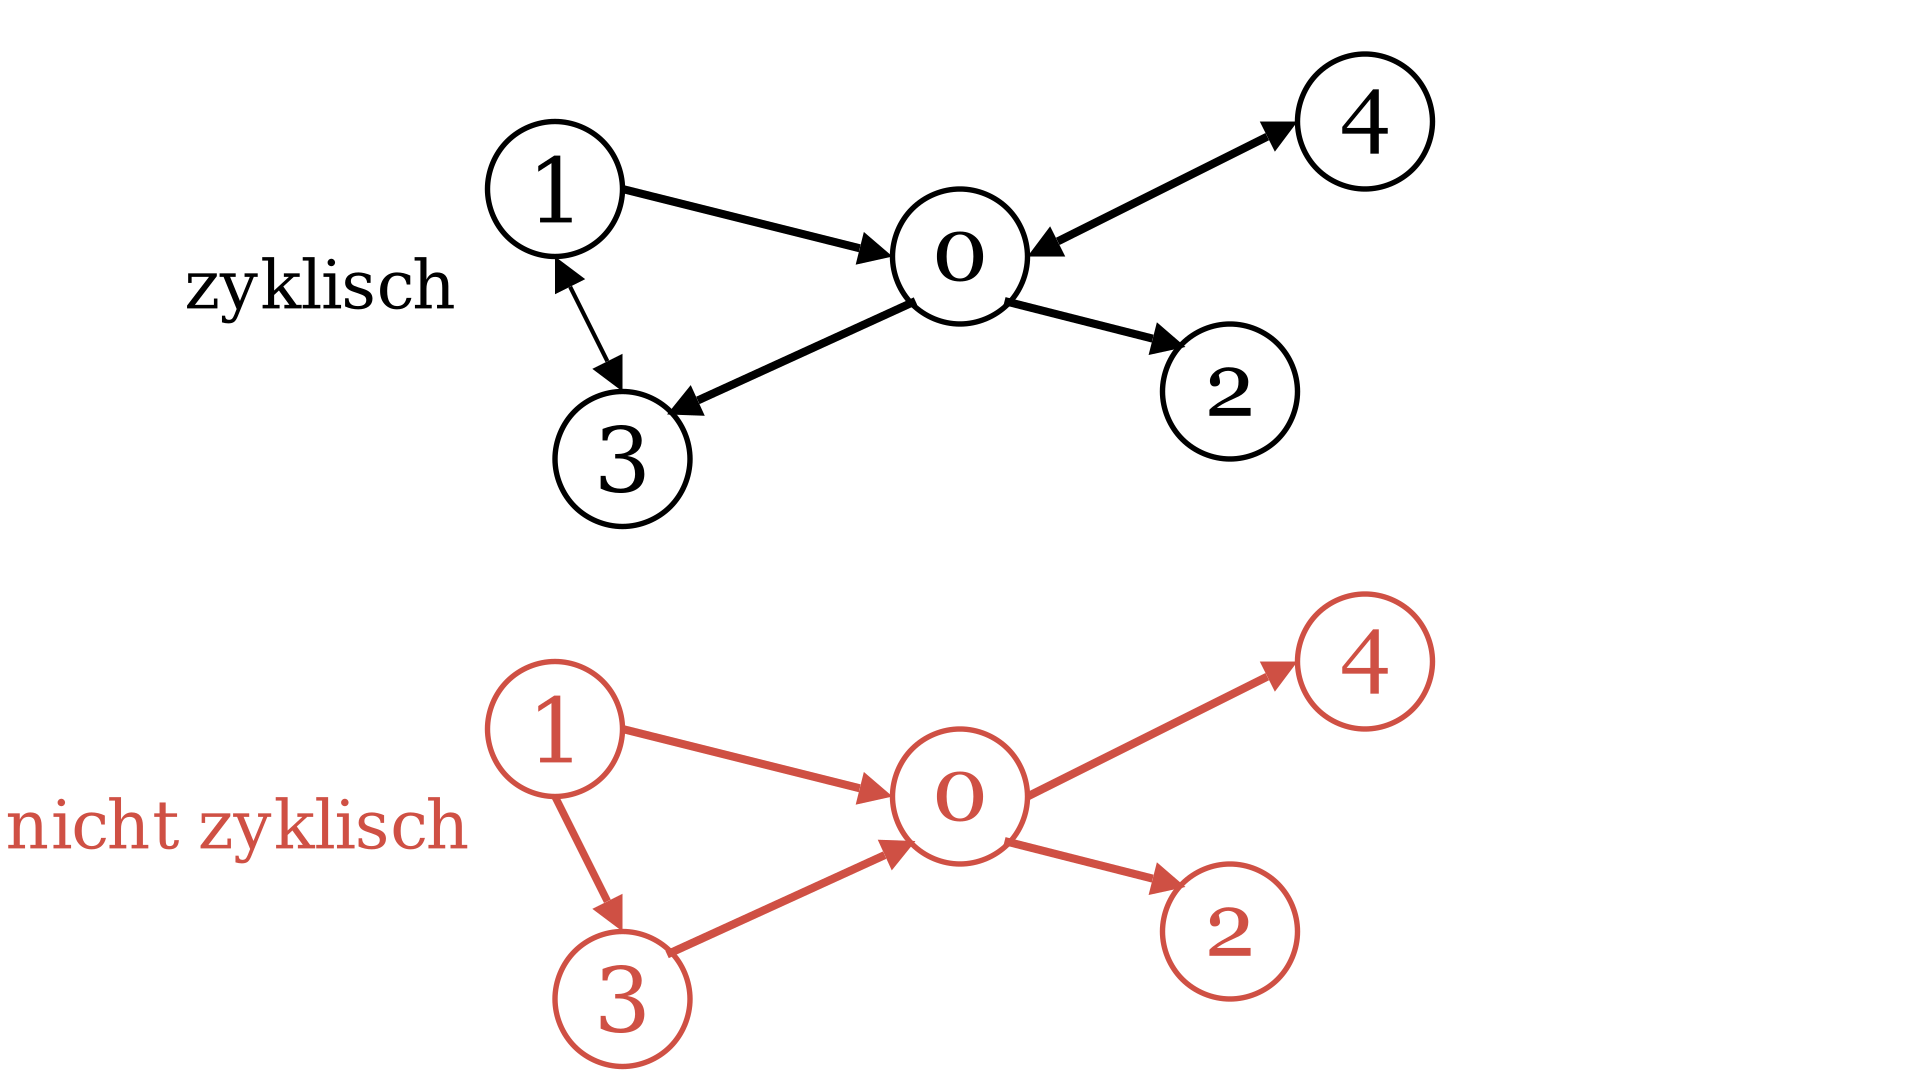
\includegraphics[scale=0.15]{../../media/zyklisch.png}
    \end{center}
    \item \textbf{zusammenhängend vs. nicht zusammenhängend}: Hier muss noch einmal weiter zwischen gerichtet und ungerichtet unterschieden werden: \\
    \textbf{ungerichtet}: hier bedeutet \textbf{zusammenhängend}, dass jeder Knoten von jedem anderen aus erreicht werden kann, d.h. für zwei beliebige Knoten $A$ und $B$ gibt es einen Pfad von $A$ nach $B$. Gibt es dagegen mindestens ein Knotenpaar, zu dem kein Pfad existiert, so ist der Graph \textbf{nicht zusammenhängend}. \begin{center}
        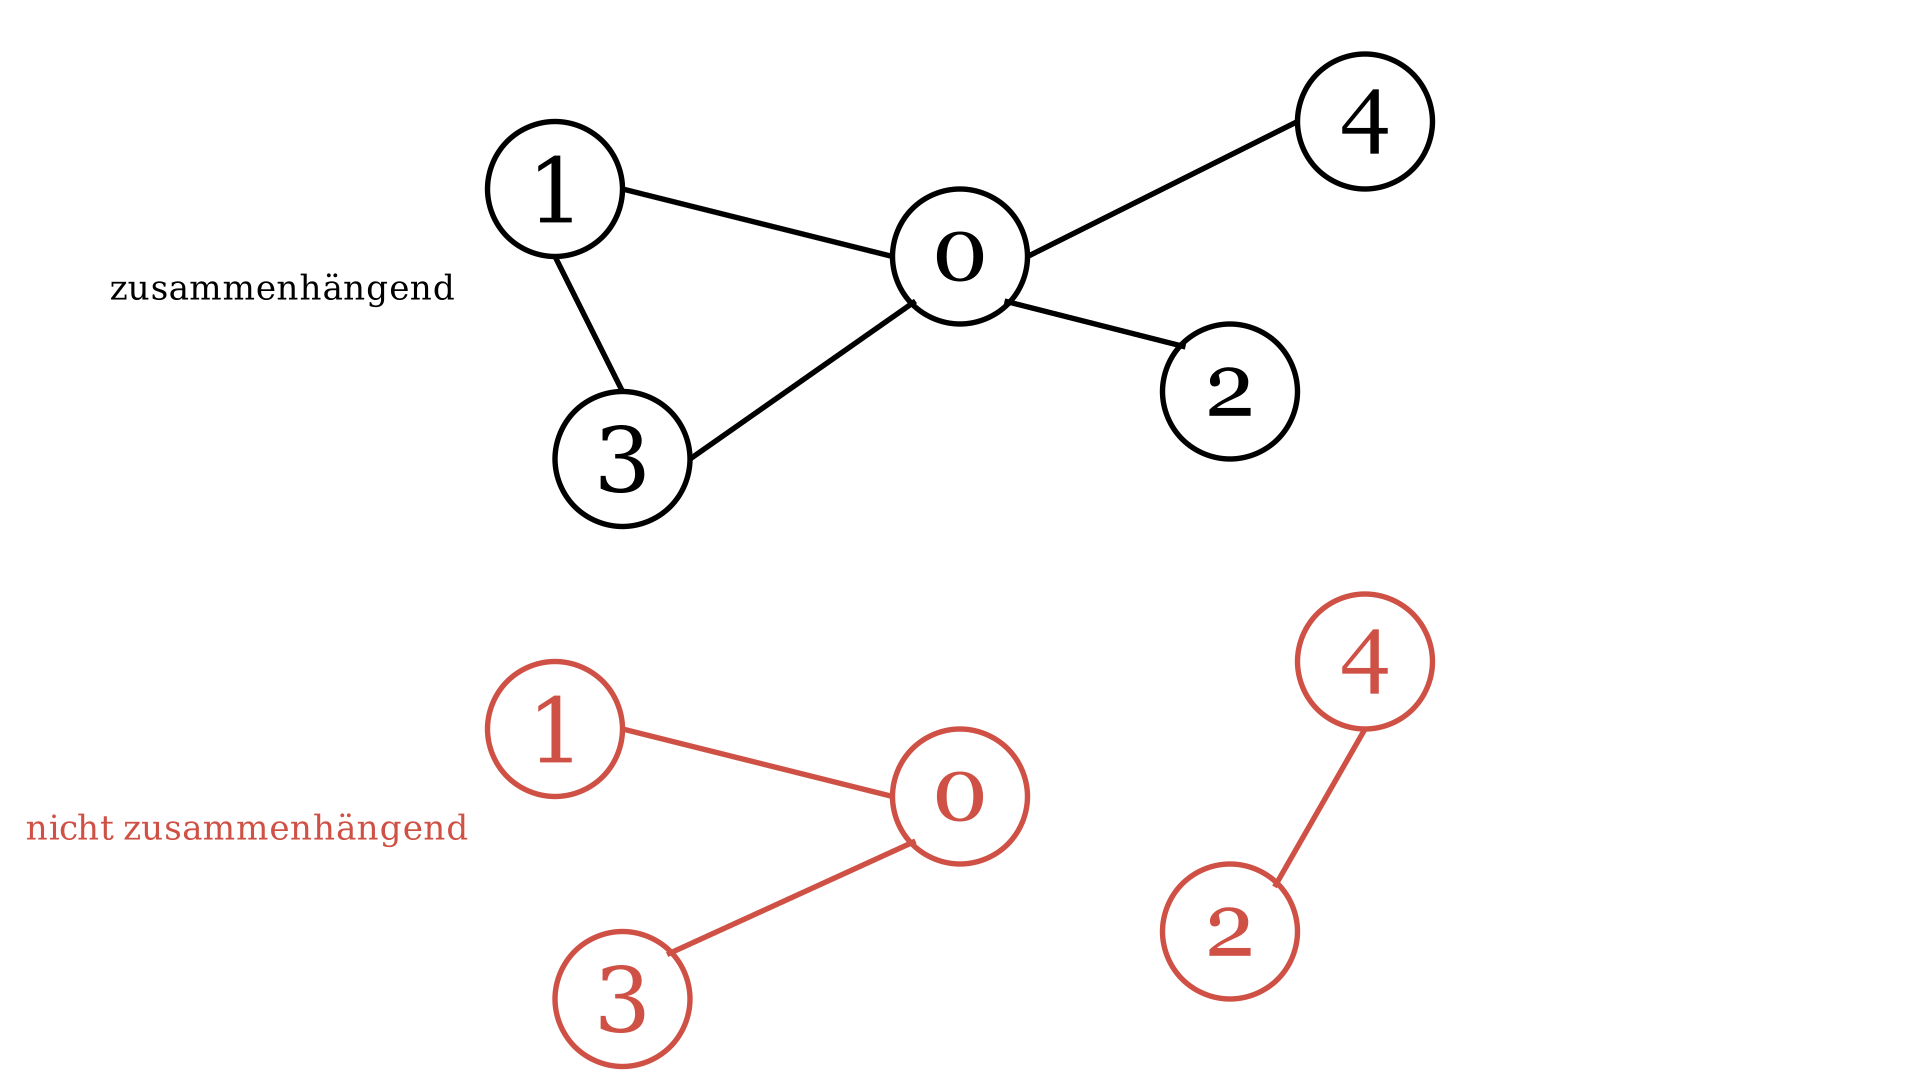
\includegraphics[scale=0.15]{../../media/ungerichtet_zusammenhang.png}
    \end{center}
    \textbf{gerichtet}: Wenn jeder Knoten von jedem anderen Knoten aus erreichbar ist, so spricht man von einem \textbf{stark zusammenhängenden} Graphen. Es wird jetzt aber noch feiner unterteilt, in beiden Fällen gilt, dass mindestens ein Knoten von mindestens einem anderen Knoten aus nicht erreichbar ist, aber:
    \begin{itemize}
        \item Interpretiert man den Graphen als ungerichtet und danach sind wieder alle Knoten von allen anderen aus erreichbar, so spricht man noch von \textbf{schwach zusammenhängenden} Graphen. 
        \item Ist auch in einem entsprechenden ungerichteten Graphen mindestens ein Knoten nicht erreichbar, so ist der ganze Graph \textbf{nicht zusammenhängend}.
    \end{itemize}
    \begin{center}
        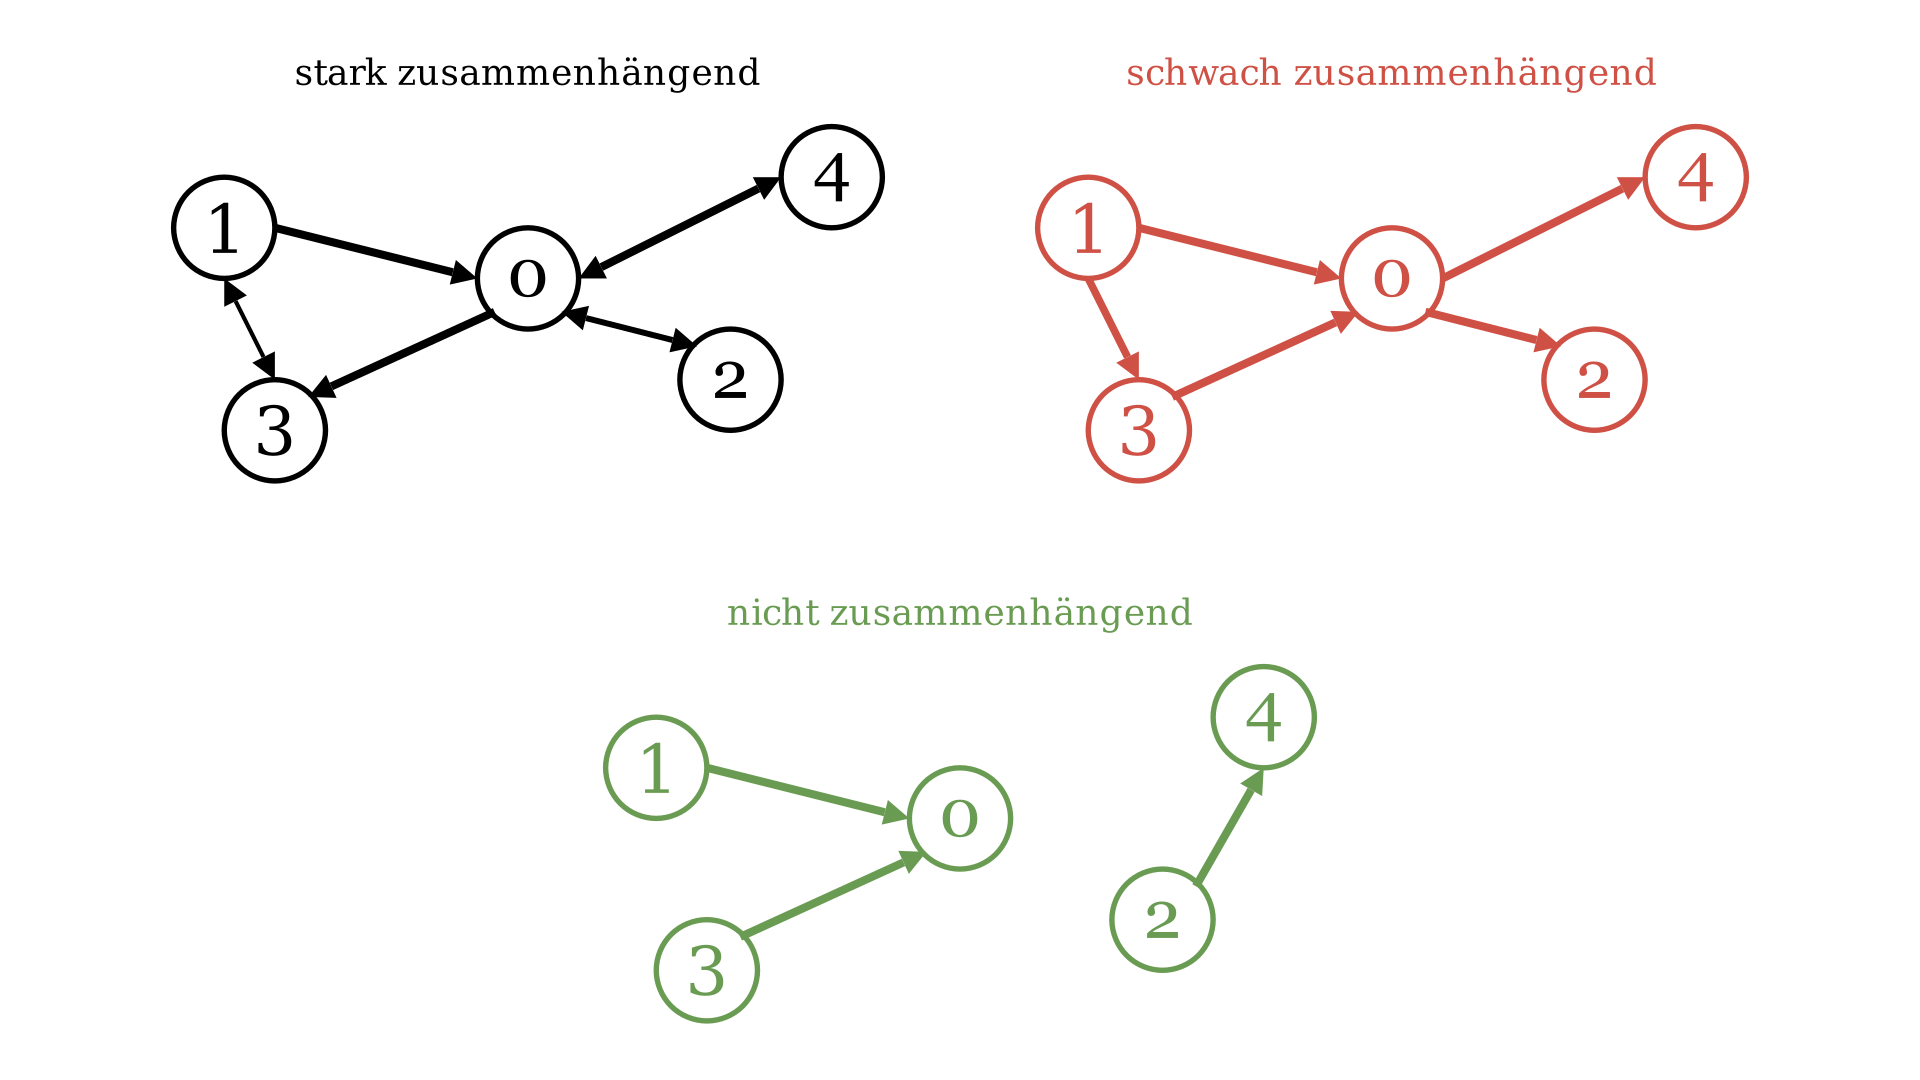
\includegraphics[scale=0.15]{../../media/gerichtet_zusammenhang.png}
    \end{center}
\end{enumerate}

\begin{task}{1}
    Klassifizieren Sie die folgenden Graphen mit möglichst vielen Fachbegriffen möglichst genau:
    \begin{center}
        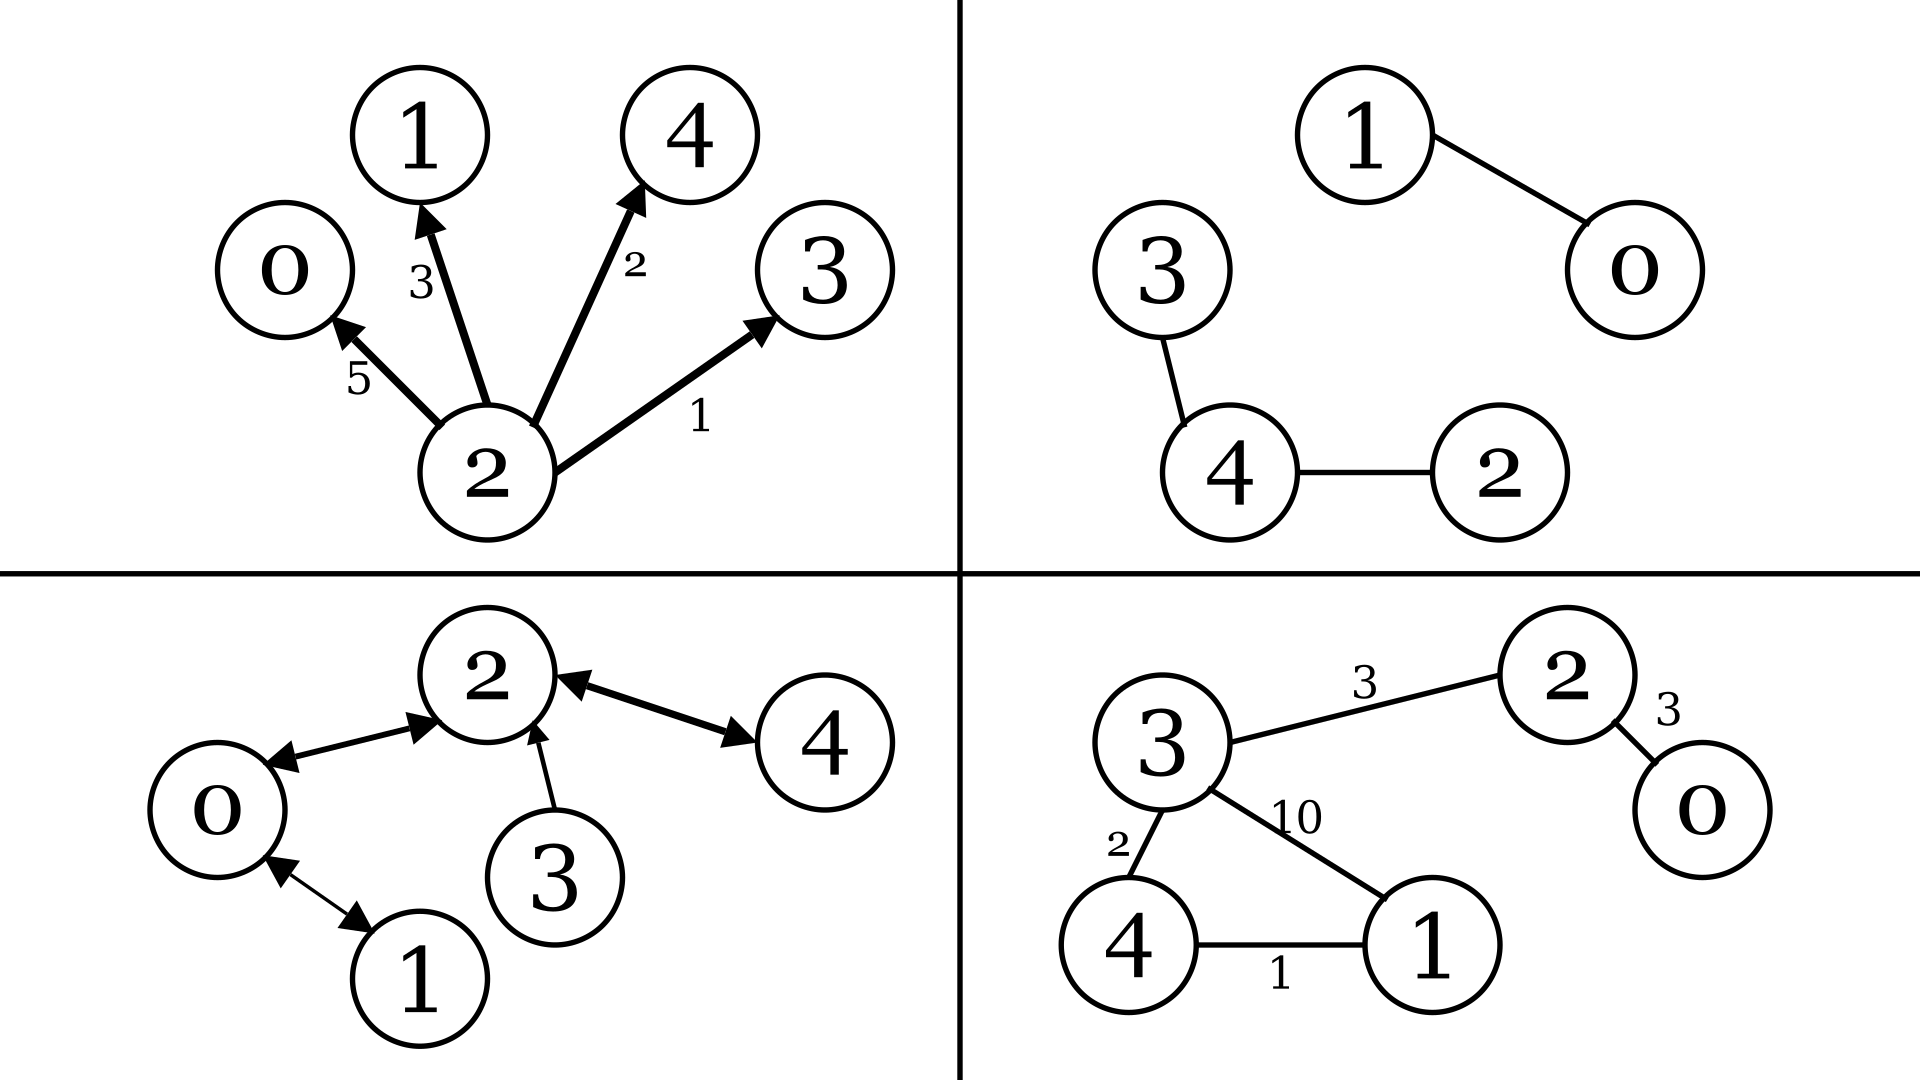
\includegraphics[scale=0.2]{../../media/graphs_task.png}
    \end{center}
\end{task}

\begin{task}{2}
    Entwefen und zeichnen Sie einen Graphen, der \dots 
    \begin{itemize}
        \item ein U-Bahn-Netz modelliert. 
        \item die Wanderwege in einem Nationalpark modelliert.
        \item ein soziales Netzwerk modelliert.
    \end{itemize}
    Verwenden Sie jeweils mindestens 10 Knoten und gegebenenfalls realistische Kantengewichte und erläutern Sie deren Bedeutung.
\end{task}

\begin{task} {3}
    Entwerfen Sie jeweils einen Graphen mit 5 Knoten und möglichst vielen Kanten bzw. Richtungen (dabei zählt jede Richtung, auch eine ungerichtete Kante zählt also als 2 Richtungen!)
    \begin{itemize}
        \item Der Graph ist ungerichtet und nicht zusammenhängend.
        \item Der Graph ist gerichtet und zykelfrei.
        \item Der Graph ist gerichtet und schwach zusammenhängend.
    \end{itemize}
\end{task}

\begin{task}{4}
Recherchieren Sie, was es mit dem \q{Vier-Farben-Satz} auf sich hat, sowie seine Verbindung zur Graphentheorie! Färben Sie anschließend eine Karte der deutschen Bundesländer passend. 
\end{task}

\begin{task}{5} 
    Überlegen Sie sich das Klassendiagramm einer eigenen Implementierung eines Graphen, orientieren Sie sich dabei an den folgenden Fragen: 
    \end{task}
    \textbf{Grundlagende Fragen/Überlegungen:}
    \begin{itemize}
        \item Welche Klassen sind nötig?
        \item Wie sollen Knoten repräsentiert werden?
        \item Wie werden die Kanten repräsentiert?
        \item Wie können Kantengewichte codiert werden?
    \end{itemize}
    Lesen Sie erst anschließend im nächsten Kapitel weiter!

\end{document}